\documentclass[10pt]{article}

\RequirePackage{nybohansenPreamble}

\usepackage[draft]{fixme}
\newcommand{\authorName}{Mads Ohm Larsen and Kasper Nybo Hansen}
\newcommand{\authorEmail}{\{omega, nybo\}@diku.dk}
\newcommand{\titleName}{Project 2}
\newcommand{\courseName}{Advanced Algorithms 2011}

\author{\authorName \\\texttt{\small{\authorEmail}}}
\title{\textsc{\titleName \\ \courseName}}
\makeindex

\begin{document}
\maketitle    

\section*{Question 1.1} % (fold)
\label{sec:question_1_1}
\paragraph{Part A} % (fold)
\label{par:part_a}

We are given a complete undirected graph $G = (V,E)$, with non-negative weights $d_{ij}$, and a viewing distance $d$. The problem is to find the shortest simple cycle so each vertex ($v_i$) is either seen or visited.

In the following we assume that the couple only wishes to visit a monument once, but possible see it multiple times. I.e. each node is visited at most once, and the cycle is thus a simple cycle. We can define the problem as follows

\begin{mydef}
Given a graph $G = (V, E)$ let a shortest cycle consist of the path $p = \{v_0, v_1,v_2,...,v_n, v_0\}$, where $v_i \in V$. Let 
\begin{equation}
  v(i) = \{j  \in V | d_{ij} \leq d\}
\end{equation}
be the set of vertices in the vicinity of vertex $i$. Let the distance between two vertices, $v_i$ and $v_j$, be calculated as
\begin{equation} 
D(v_i,v_j) = 
\begin{cases}
 d_{ij} &  \quad d_{ij}>d \\
 0      &  \text{otherwise}
\end{cases} 
\end{equation} 

The path $p$ should be chosen so 
\begin{equation}
  \forall v \in V : \exists v_i \in p : v \in v(v_i) 
\end{equation}        

The vertices in $p$ and their ordering should be chosen so the following function is minimized
\begin{equation}
  D(p[0],p[n])+\sum_{i=0}^{n-1} D(p[i],p[i+1])
\end{equation}

where $p[i]$ is the $i'th$ vertex in the path $p$.
\label{def1}
\end{mydef}

Transforming the above definition into a decision problem yields: Given a graph $G$, view distance $d$ and a number $l$ is there a cycle of length at most $l$, which satisfy the above.

The corresponding language is

\begin{align*}
   \text{TCP_cycle} = \{ \langle G, d, l \rangle : &G = (V,E) \text{ complete undirected graph},\\ 
                                                   &d = \text{Viewing distance}  \\
                                                   &l = \text{Length of tour}  \}
\end{align*}

% paragraph part_a (end)

\paragraph{Part B} % (fold)
\label{par:part_b}
We need to show that the TCP problem is NP-complete. In order tho show that the TCP problem is NP-complete, we need to show that $TCP \in NP$ and that it is NP-complete. 

$TCP$ is in NP if we can come up with a polynomial time algorithm that given a cycle and a graph, can answer yes if the cycle is indeed a TCP cycle otherwise no. Such an algorithm could be. Given a graph $G=(V,E)$ and a cycle $P$, verify that each vertex $v \in V$ is visible by at least one vertex in $p \in P$. This verification could indeed be implemented to run in polynomial time, yielding $TCP \in NP$.

$TCP$ is NP-complete if we can show $HAM-CYCLE \leq TCP$. Thus if we can use $TCP$ to find a hamilton circle, we have shown that $TCP$ is NP-complete. Let $G = (V, E)$ be an instance of the Hamilton cycle problem. We can transform this problem into a $TCP$ problem, by the following transformation. Let $G' = (V, E')$ be a fully connected graph, where $E' = \{(u,v) : u,v \in V \wedge u \neq v\}$, and each edge, $(u',v') \in E'$, has a distance as follows

\begin{equation} 
d(u',v')  = 
\left\{
\begin{array}{rl} 
  1 & (u',v') \in E\\
  0 & (u',v') \notin E\\ 
\end{array} 
\right. \qquad \forall (u',v') \in E'
\end{equation} 
Now run the $\text{TCP_cycle}$ algorithm on $G'$ and let $d=0$ and $l = |V|$. Now $G$ has a Hamilton cycle if and only if the $\text{TCP_cycle}$ returns true.

The time complexity of the $TCP$ problem is at least as hard as the $HAM-CYCLE$ problem (stated differently a solution to $HAM-CYCLE$ is at least as easy as a solution to $TCP$). We thus assume that no polynomial time algorithm exists for the problem.

% paragraph part_b (end)
% section question_1_1 (end)

\section*{Question 1.2} % (fold)
\label{sec:question_1_2}

\begin{figure}
	\centering
	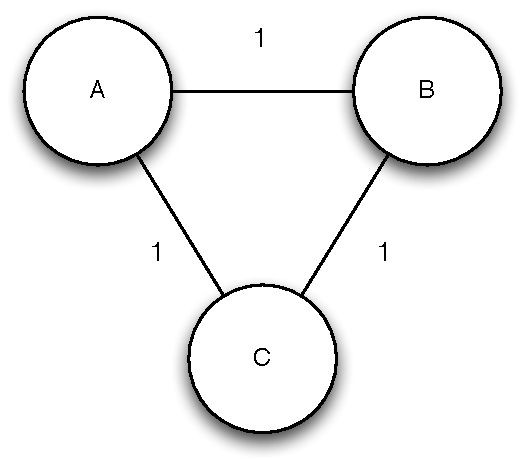
\includegraphics[width=0.4\textwidth]{figures/unicycle.pdf}
	\caption{A graph where the smallest 1-tree is larger than the optimal TCP cycle. $d \geq 1$}
	\label{unicycle}
\end{figure}
In figure \ref{unicycle} we have depicted a set of points $A$, $B$ and $C$, in which the smallest 1-tree, $A-B-C$ is larger than the optimal TCP cycle, which can be one of the three points.
The $d$ value is in this instance greater or equal to $1$.
% section question_1_2 (end)

\section*{Question 1.3} % (fold)
\label{sec:question_1_3}
First lets define the function $v(i)$ to be
\begin{equation}
   v(i) = \{ j \in V\ |\ d_{ij} < d \}
\end{equation}

In the following \texttt{ILP} definition of the problem, $x_{ij}$ denotes the usage of an edge from $i$ to $j$.
Likewise, $y_i$ denotes the usage of vertex $i$.
\begin{align}
\min &\qquad \sum_{(i,j) \in V^2} d_{ij} x_{ij} \\
s.t. &\qquad \sum_{i \in v(j)} y_i \geq 1 \quad \forall j \in V \\
	 &\qquad \sum_{(i,j) \in Z^2} x_{ij} \leq \sum_{i \in Z} y_i \quad \emptyset \subset Z \subset V \label{st1}\\
	 &\qquad \sum_{j \in V } x_{ij} - 2 y_i = 0 \quad \forall i \in V \\
	 &\qquad y_i \in \{0,1\}, \quad x_{ij} \in \{0,1\}  \label{st2}
\end{align}

% section question_1_3 (end)

\section*{Question 1.4} % (fold)
\label{sec:question_1_4}
In order for the ILP formulation to become a lower bound, we can remove the constraint (\ref{st1}) and relax the constraint (\ref{st2}) so $y_i \geq 0$ and $x_{ij} \geq 0$.
% section question_1_4 (end)

\section*{Question 2.1} % (fold)
\label{sec:question_2_1}
We have implemented the lower-bound method by removing and relaxed the constraints as explained in question 1.4. For details of the implementation see attached file \texttt{BnB.java}. 
% section question_2_1 (end)

\section*{Question 2.2} % (fold)
\label{sec:question_2_2}
  
% section question_2_2 (end)

%\section*{Question 2.3} % (fold)
%\label{sec:question_2_3}
% Optional
% section question_2_3 (end)


%\bibliographystyle{abbrv}
%\bibliography{bibliography}

\end{document}                      



